\section{Method}
In this paper the system used to describe the the interactions in a multi-domain
environment is a directed graph.
Therefore form the beginning of the design process when each component, 
like part specific functions are briefly defined, till to the cleaned up and summarized endproduct,
each step of the process have to described in the same manner.
This requires the ability to subdivide, summarize and outsource functionalities. 
Each function is blackbox with unknown system behavior, but known input and output values.
Therefor each system needs to implement a certain interface, 
which allows to control the system behavior with input data and options.
Additionaly, each step of the workflow needs an update mechanism to update the outputs accordingly.
The resulting entity with inputs, outputs, options and an update mechanism is further called a 'node'.\\
A system is build by connecting the output and input values of a two nodes.
The resulting dependencies can build complex interactions with multiple loops and multiple branches.
These systems are very similar to modern programming languages which are proven to be Turing-Complete.
This means, that no algorithm can be developed which can determine if the system will converege to a solution.
Therefore further approximations are introduced:
\begin{enumerate}
    \item the system does not converged, when after n solving runs the outputs values still change
    \item a output value is changed if the value differes from the previous update call
    \item a solver run is done if every node is updated at least once
\end{enumerate}

\begin{algorithm}[bt]
    \KwIn{List of Processes\\
    Priority $\in$ ["manual", "dynamic", "time"]}
    \KwOut{Updated and converged processes}
    sort(List of Processes)\;
    \textbf{set} GState to "changed"\;
    \textbf{set} StartPos to 0\;
    \While{GState = "changed"}{
        \textbf{set} GState to "unchanged"\;
        \For{i = StartPos to sizeof(List of Processes)}{
            \textbf{set} CurrProcess as ith Element of List of Processes
            \textbf{set} GState to "unchanged"\;
            \textbf{set} STime to currentTime()\;
            \textbf{set} PState to CurrProcess.update()\;
            \textbf{set} ETime to currentTime()\;
            \textbf{set} $\Delta$Time to ETime - STime\;
            \If{Priority equals "time"}{
                CurrProcess.Time = round($\log_{10}${$\Delta$Time})\;
            }
            \If{PState equals "changed"}{
                \textbf{set} GState to "changed"\;
            }
            \If{CurrProcess.Inputs equals 0 \emph{\textbf{and}} Priority not "manuel"}{
                \textbf{set} StartPos to i\;
            }
            \If{Priority equals "dynamic" \emph{\textbf{or}} Priority equals "time"}{
                \textbf{set} List of FProcesses as List of Processes starting from CurrProcess\;
                \ForEach{FurtherProcess in  List of FProcesses}{
                    FurtherProcess.InputChanges.update()\;
                }
                sort(List of FProcesses)\;
            }
            increase i by one\;
       }
    }
\caption{\label{code:update-standard-processor}Update-Algorithm for complex systems}
\end{algorithm}
With this simplifications it is possible to uses the heuristic approach (algorithm \ref{code:update-standard-processor}) to approximate the solution.
However this approach requires a intelligent ranking of the nodes.
Therefor the following rules are introduced:
\begin{enumerate}
    \item nodes with no connected inputs are starting points and should always be at the beginning of a update progress
    \item nodes which needs more time to compute should update as rarely as possible
    \item nodes where a majority of all inputs have already changed have priority
    \item nodes with fewer connections have lesser dependencies and therefor have priority
\end{enumerate}
The rule based sorting algorithm \ref{code:sort-process} is therefor constantly used during the updating process.
\begin{algorithm}[ht]
    \SetAlgoLined
    \KwIn{list of porcesses}
    \KwOut{sortet list of processes}
    use bubble sort to sort the list\; 
    \Fn{\FBSort{Process A, Process B}}{
        \eIf{A.InputConnections == B.InputConnections}{
            \eIf{A.Time == B.Time}{
                \eIf{A.InputConnections-A.InputChanges == B.InputConnections-B.InputChanges}{
                    \eIf{A.InputChanges == B.InputChanges}{
                        \Return{A.OutputConnections $<$ B.OutputConnections}
                    }{
                        \Return{A.InputChanges $>$ B.InputChanges}
                    }
                }{
                    \Return{A.InputConnections-A.InputChanges $<$ B.InputConnections-B.InputChanges}
                }
            }{
                \Return{A.Time $<$ B.Time}
            }
        }{
            \Return{A.InputConnections $<$ B.InputConnections}
        }
    }
    \textbf{end}
\caption{\label{code:sort-process}Sort-Algorithm}
\end{algorithm}
The sorting of the second algorithm can be 
test
\begin{figure}[h]
    \centering
    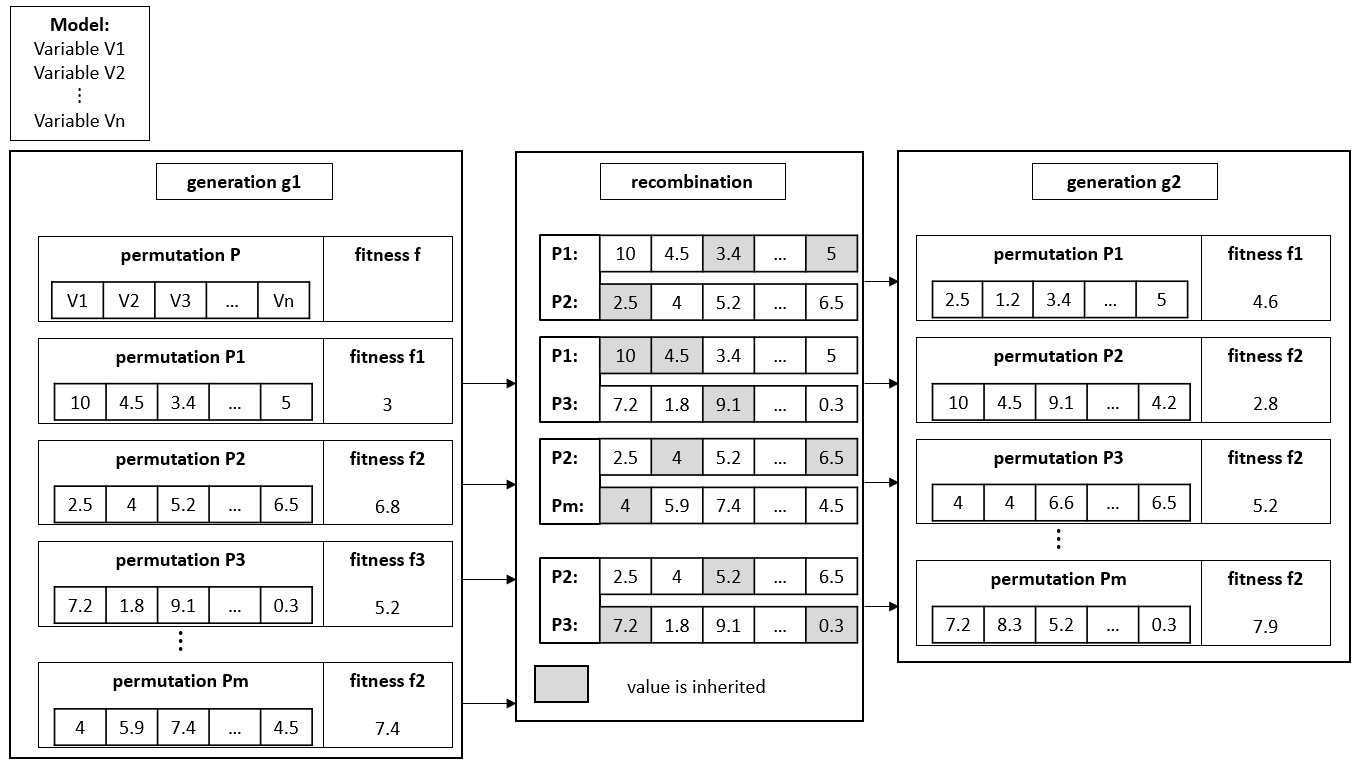
\includegraphics[scale=0.5]{pics/evol_alg.PNG}
    \caption{\label{pic:evol_alg} "General approach for development and construction (VDI 2221)." \cite{Jansch2006THEDO}}
\end{figure}\\
test
